\documentclass[11pt]{article}
\usepackage[utf8]{inputenc}
\usepackage[T1]{fontenc}
\usepackage{amsmath}
\usepackage{amsfonts}
\usepackage{amssymb}
\usepackage[version=4]{mhchem}
\usepackage{stmaryrd}
\usepackage{graphicx}
\usepackage[export]{adjustbox}
\graphicspath{ {./images/} }
\usepackage{hyperref}
\hypersetup{colorlinks=true, linkcolor=blue, filecolor=magenta, urlcolor=cyan,}
\urlstyle{same}

%New command to display footnote whose markers will always be hidden
\let\svthefootnote\thefootnote
\newcommand\blfootnotetext[1]{%
  \let\thefootnote\relax\footnote{#1}%
  \addtocounter{footnote}{-1}%
  \let\thefootnote\svthefootnote%
}

%Overriding the \footnotetext command to hide the marker if its value is `0`
\let\svfootnotetext\footnotetext
\renewcommand\footnotetext[2][?]{%
  \if\relax#1\relax%
    \ifnum\value{footnote}=0\blfootnotetext{#2}\else\svfootnotetext{#2}\fi%
  \else%
    \if?#1\ifnum\value{footnote}=0\blfootnotetext{#2}\else\svfootnotetext{#2}\fi%
    \else\svfootnotetext[#1]{#2}\fi%
  \fi
}

\begin{document}
Exit Strategies for Private Equity Investments

Venture capital and buyout funds can exit investments, or raise cash without an exit, using one or more of the following methods:

\begin{enumerate}
  \item Sale to a strategic buyer: A strategic merger is the most common exit strategy for private companies, which takes place when the private company is sold to an operating company in the same or adjacent industry. A strategic merger may be preferred, because the proceeds of a strategic merger may be able to be liquidated more quickly than an IPO, where publicly traded shares may be subject to a lockup period.

  \item Initial public offering (IPO): If the underlying company would make an attractive stand-alone publicly traded company, an investment bank could be retained to take the firm public.

  \item Another LBO or leveraged recapitalization: The firm could be refinanced by the current owners using another LBO deal, in which debt is reintroduced into the company to compensate management for its equity stake. In fact, the existing management team may even remain the operators of the company with an existing stake in the second LBO transaction, providing them with the opportunity for a second round of leveraged equity appreciation. In this transaction, proceeds of the debt are used to purchase shares of the company from the sponsor of the initial LBO.

  \item Buyout-to-buyout deal: Buyout-to-buyout deals are increasingly common in the private equity industry. A buyout-to-buyout deal, also known as a secondary buyout or financial merger, takes place when a private equity firm sells one of its portfolio companies to another buyout firm or a financial investor. The second buyout firm believes that it can create a second leg of growth after the original buyout firm sells the company. It is estimated that approximately one-half of private equity deals are now buyout-to-buyout deals. Initially, secondary buyouts were rare. Private equity firms were reluctant to sell a portfolio company to another private equity firm in a buyout-to-buyout deal because of the stigma of failure associated with not being able to take a company public or sell it to a strategic partner. Increasingly, private equity firms are selling to one another as an exit strategy. This strategy is frequently used when a private equity fund that is winding down its life (years 8-12) sells to another private equity fund earlier in its life cycle (years 1-5).

  \item Direct listing: While an IPO seeks to raise new capital and results in a listing of a newly traded public company, a direct listing achieves the same publicly traded status without employing an underwriter. In a direct listing, existing shareholders, including the company, the company's employees, or the private equity fund, convert their privately held shares into publicly traded shares that are listed on an exchange. The shareholders simply exchange their private shares for publicly traded shares and may choose either to hold or to liquidate those shares in the public market. Historically, direct listings simply listed existing shares without raising new capital, but more recent direct listings have been able to sell new shares to raise capital.

  \item Special purpose acquisition corporation (SPAC): A special purpose acquisition company (SPAC) is a publicly traded "blank-check" company that is formed for the purpose of completing an acquisition of a private company and allowing the acquired company to assume the SPAC's public listing. The SPAC floats an IPO to raise capital and uses the proceeds of the IPO and additional capital sources to purchase a private company.

\end{enumerate}

While IPOs were the majority of portfolio company exits from buyout funds in most of the 1990s, IPOs comprised around $10 \%$ of exits in the 2010 s. In recent years, there has been a substantial increase in the portion of exits attributed to secondary buyouts. Similarly, over $90 \%$ of venture capital-backed companies exited through mergers over the last decade compared to over $80 \%$ of exits through IPOs in the 1980s.

\begin{center}
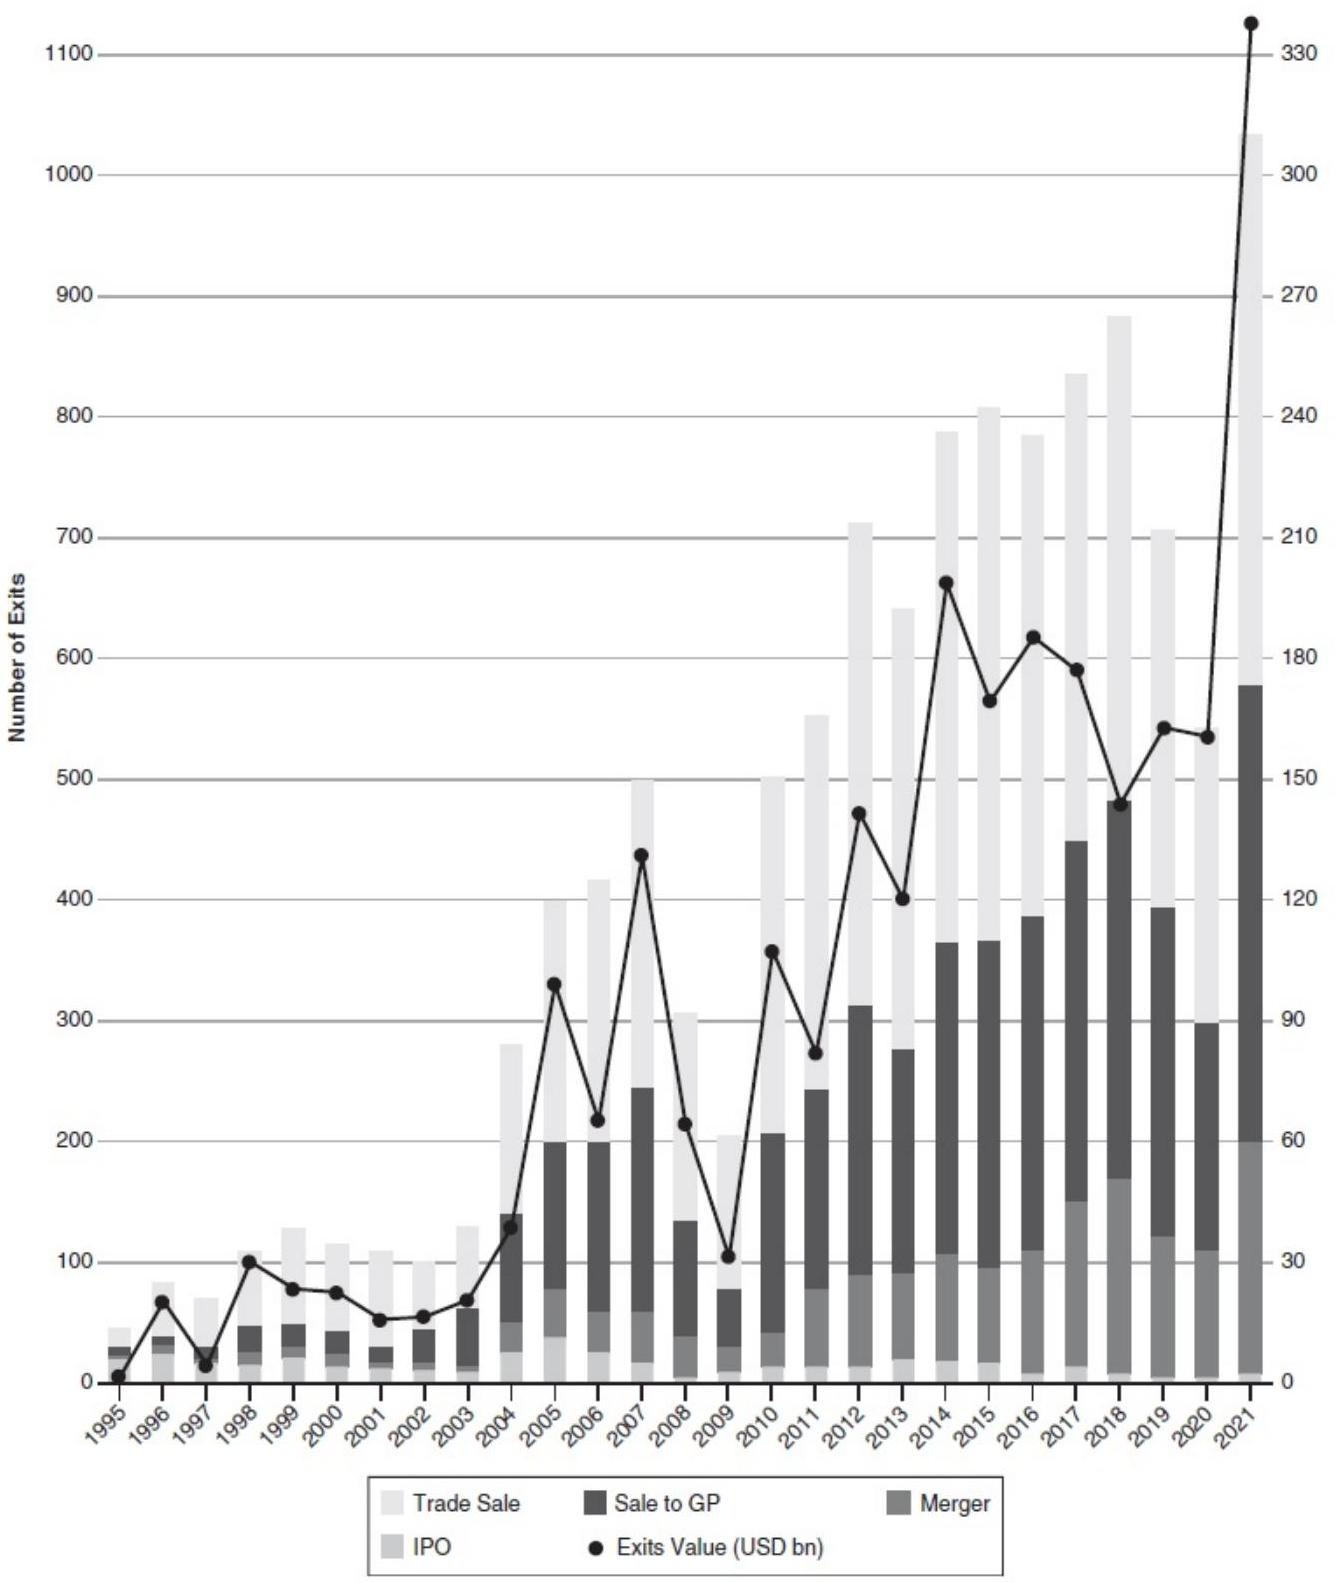
\includegraphics[max width=\textwidth]{2024_04_10_a5ce63565cca064665e9g-3}
\end{center}

Buyout Capital Backed Exits by Exit Type, 1995-2021

Source:Preqin\\
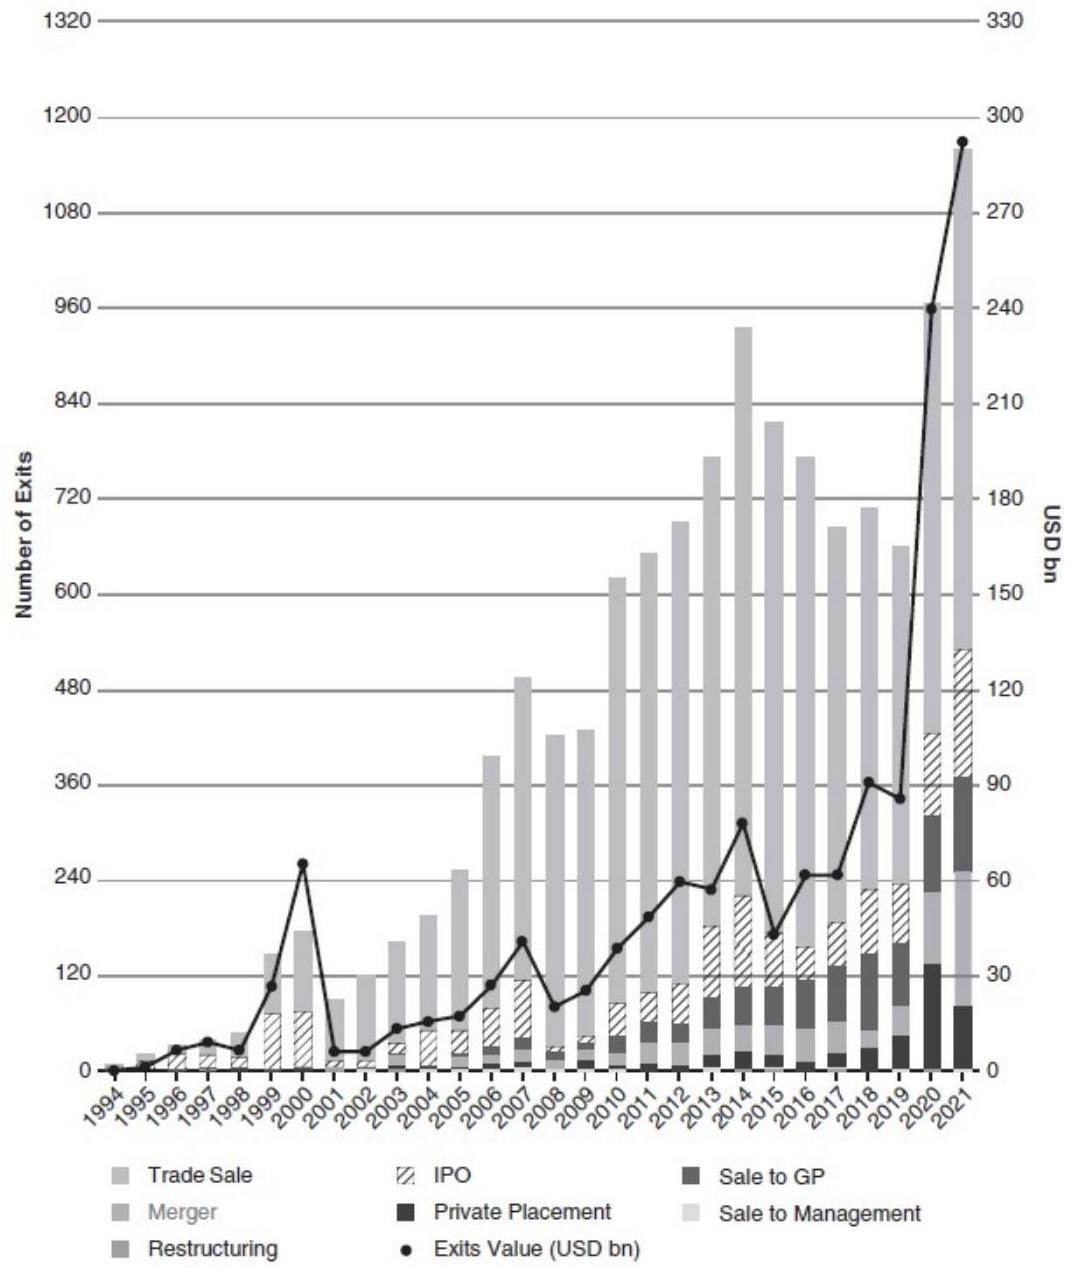
\includegraphics[max width=\textwidth, center]{2024_04_10_a5ce63565cca064665e9g-4(1)}

Venture Capital Backed Exits by Exit Type, 1994-2021

Source:Preqin

\section*{Initial Public Offerings}
In an initial public offering (IPO), private companies are taken public by selling shares for the first time in the public markets. By selling newly issued shares, the company is able to raise capital for corporate purposes such as acquisitions or capital expenditures. Note, in the exhibit Venture Capital-Backed IPOs and Median Time to IPO, that the median age of companies offering initial public offerings was 4.5 years or less from 1996 to 2001, while increasing from 6.2 years to 7.8 years from 2006 to 2016. This trend suggests a maturation of private markets, which are providing capital on a larger scale to a larger number of companies, delaying or eliminating the need for companies to go public just to meet capital needs. By 2021, VC-backed IPOs reached their highest levels since 2000, with Median Time to IPO declining to 6.0 .

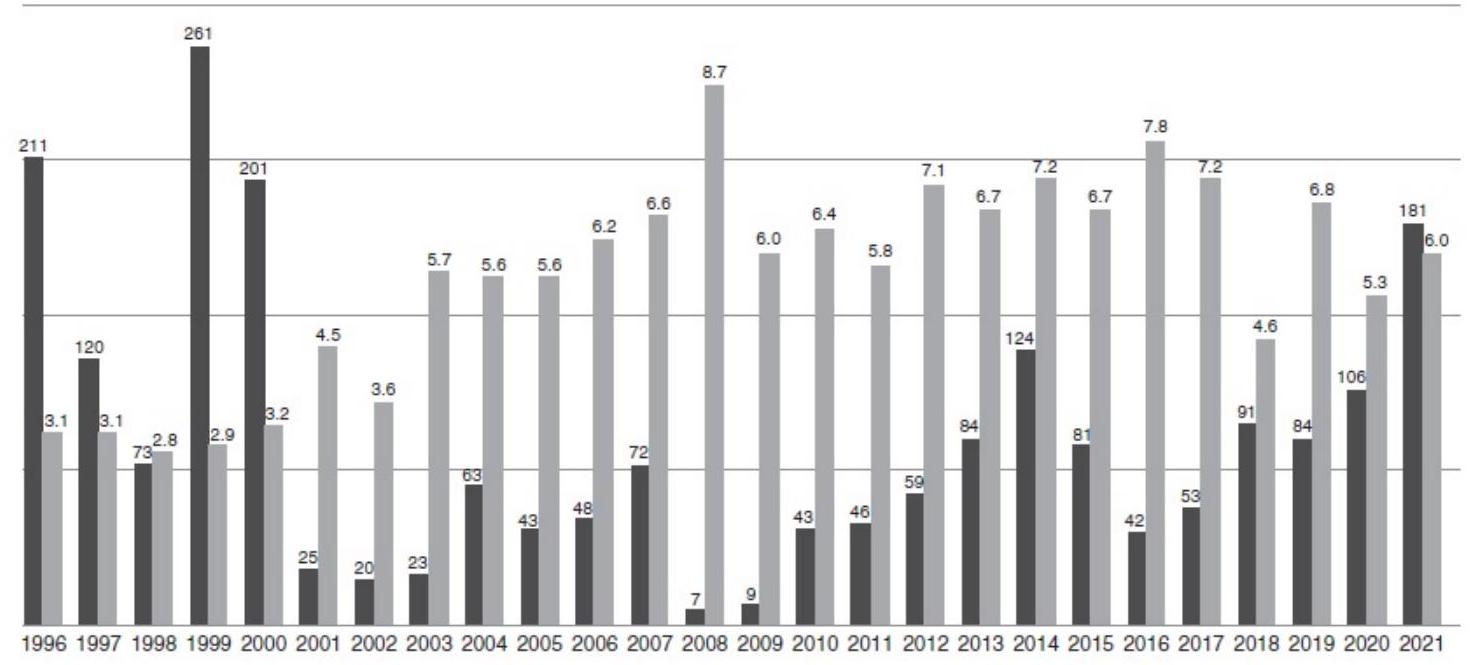
\includegraphics[max width=\textwidth, center]{2024_04_10_a5ce63565cca064665e9g-4}
\footnotetext{\begin{itemize}
  \item \# of deals $\quad$ Median time from initial equity funding to IPO (in years)
\end{itemize}
}

Source: NVCA

The above chart is based on US IPOs by VC-backed US issuers.

As with all newly public companies, the company must provide transparency to investors, such as by publishing quarterly financial statements, an annual report, and required regulatory filings. In the US, the costs of being a publicly traded company are seen as significant, with the result being that IPO activity has declined by almost $60 \%$ since the 2002 implementation of the Sarbanes-Oxley regulations. This decline in IPO activity is noted in the exhibits Evolution of Exits for US Buyouts, 1985-2019 and Evolution of Exits for US Venture Capital, 1980-2019. In reaction to fraudulent financial statements by publicly traded companies in the early 2000s, these regulations now impose criminal penalties on corporate officers, such as CEOs or CFOs, who release inaccurate financial statements. The regulation also strengthened requirements for internal controls and processes that auditors and accountants must follow when assisting with the preparation of those financial statements. Hartman (2006) ${ }^{1}$ The Costs of Being Public in the Era of Sarbanes-Oxley, Thomas E. Hartman, Foley and Lardner, LLP, June 2006. notes that in the first four years after the passage of Sarbanes-Oxley, public companies with under $\$ 1$ billion in annual revenue saw annual compliance costs increase by $174 \%$. The IPO Task Force (2011) ${ }^{2}$ Rebuilding the IPO On-Ramp, IPO Task Force, October 2011, presentation to US Department of the Treasury. noted that the regulatory cost of an IPO is $\$ 2.5$ million followed by annual compliance costs of $\$ 1.5$ million. These fixed annual costs for attorneys, accountants, auditors, and exchange fees may be prohibitively expensive for smaller companies, likely preventing companies from going public below a market capitalization of $\$ 50$ million.

Going public by issuing an IPO has a very specific process, which may take three to six months or even longer to complete. The process includes following all regulatory requirements as well as arranging for a large number of new investors to allocate capital to the newly public firm. At the beginning of this process, there is no guarantee that the company will go public, especially if market conditions change. Many companies will go public when the IPO window is open, a time at which the public market is receptive to purchasing shares in newly public companies at high prices. The ability of companies to go public may vary over time, with IPOs more likely when public market returns are strong and less likely when equity markets are experiencing declines and high levels of volatility. The IPO window may be more or less favorable at a given time depending on the industry in which a company operates. For example, there may be times where it is relatively easy to sell growth companies in the biotech or computer technology industries at high levels of valuation, even when, at the same time, it might be difficult to sell value companies in the energy or industrial sectors at any level of valuation.

The company will hire an underwriter, which is an investment bank that will oversee the IPO process and solicit new investors to purchase the public securities of the firm. The underwriter receives fees for their services, up to $7 \%$ of proceeds for smaller companies and $4 \%$ or less for larger companies. Extremely large companies, such as Saudi Aramco, have been able to go public for an underwriter's fee of as little as $1 \%$.

The first step is to draft a prospectus, where the company, working with attorneys, investment banks, and accountants, files disclosures with the national market regulator; in the US the Securities and Exchange Commission (SEC). The prospectus includes company details such as the historical financial statements, an overview of the firm's business model, and the company's competitive strengths and growth strategy, as well as material risk factors, among other characteristics. If this prospectus does not disclose all material information regarding the firm, it might be rejected by the regulator or may expose the company to future litigation should undisclosed factors lead to a decline in the stock price. Note that the prospectus only contains information on the current state of the company as well as its historical financials. Once the IPO prospectus is filed with regulators, the company and their underwriter(s) have a quiet period where they can't discuss the company's financials and prospects until the prospectus is approved. A second quiet period of ten days starts from the date of the IPO.

Once the regulator declares the IPO prospectus to be acceptable, the company and the underwriter embark on a road show to pitch the company to potential investors and build an order book of demand at various prices. The company and its underwriters are not allowed to make projections regarding future financials of the firm in either the prospectus or the road show. During this book-building process, the underwriter receives indications of interest from investors regarding the price they would pay for each share as well as the number of shares they have an interest in purchasing. The underwriters have a goal of having the IPO be oversubscribed, where there is demand to purchase a larger number of shares than the company is planning to sell.

The company may target a specific market capitalization, which is the price per share multiplied by the number of shares outstanding. For example, a company will have a $\$ 2$ billion market capitalization if they have 100 million shares outstanding at a price of $\$ 20$ per share. Note that many IPOs will sell only a small portion of the company's shares outstanding, such as $10 \%$ to $20 \%$. In this example, the company would sell 20 million shares in the primary offering at $\$ 20$ per share, raising $\$ 400$ million from new shareholders before the costs of the offering. After paying the underwriting fees, the cash is returned to the company as cash to hold on the balance sheet, to reduce debt, to make acquisitions, or for capital expenditures. The remaining 80 million shares would be retained by employees, private equity firms, and institutional investors, or reserved by the company for future secondary offerings.

In order to sell 20 million shares at $\$ 20$ each, the underwriter may wish to solicit bids for 40 million shares, which would make the IPO $100 \%$ oversubscribed. The larger degree of oversubscription to the IPO, the more likely the company will successfully raise the required capital and perhaps have a strong increase in the stock price during the first day of trading. The actual price of the IPO is set the night before the stock is to begin trading as a public company. Until the final price is set, there is considerable uncertainty as to what the final price will be and even if the IPO will happen. There are numerous examples of companies failing to go public even after completing a road show and all of the regulatory requirements. If there is not sufficient demand for the shares to accomplish the fundraising goals of the firm, the IPO may be cancelled or postponed until a time when investors are willing to purchase the shares at the company's preferred price and quantity.

Some market participants worry about a "first-day pop," where those buying shares in the IPO paid the $\$ 20$ IPO price, while investors buying on the first day of public trading may pay $\$ 25$ or more per share. If the stock price closes the first-day at $\$ 25$, all of the investors buying directly from the underwriter experience a $25 \%$ gain, while the company sold shares at a price below where they were valued in the market at the end of the first-day. While some are worried that this enriches IPO investors at the cost of the company and those buying shares in the public market, this first-day pop can actually be positive for the company. If the IPO was priced to provide a smaller first-day return, it might be more difficult to attract investors to the IPO and the deal might not be successful at raising the required amount of capital and meeting the company's goal of becoming publicly traded. The first-day price increase can attract media and investor attention, which generates free publicity for the company and creates a new class of shareholders. Also note that, in this example, the company only sold $20 \%$ of its authorized shares. After a lockup period of 90 to 180 days, those owning private shares, such as employees and private equity firms who did not sell their shares in the IPO, are allowed to sell their shares in the public market. This three to six months of trading has established a market price and liquidity that will allow private investors to sell their holdings at what may be an equilibrium price. After the IPO, the company can issue new shares in many ways, such as for employee compensation, mergers and acquisitions, or as secondary stock offerings where corporate owned shares are issued into the public market for a new cash infusion.

\section*{Direct Listings}
A direct listing can be a cheaper and faster way for a company to become publicly traded, but has historically lacked the ability to raise new capital. In a direct listing, existing shares in the private company are converted into publicly traded shares. Those shares newly available as public securities may have been owned by the\\
company or employees as well as institutional investors and private equity funds. Direct listings may lack a lockup period, so the owners of the private shares are able to sell their holdings as soon as the publicly listed shares start trading.

At the end of 2020, regulations in the US evolved to allow direct listings to raise new capital without the assistance of an underwriter, also called primary direct listings. This change will make it cheaper for companies to go public, but the SEC has expressed concerns about investor protection when an underwriter is not involved in the process. ${ }^{3}$ Statement on Primary Direct Listings, \href{https://www.sec.gov/news/public-statement/lee-crenshaw-listings-2020-12-23}{https://www.sec.gov/news/public-statement/lee-crenshaw-listings-2020-12-23}

While the direct listing may be cheaper and easier, it must be noted that the company will not typically have the services of an investment banker or an underwriter. Not only are the underwriters helpful in the process of setting a valuation, raising capital, and attracting new investors, but they may also support the newly public stock through research coverage, credit support, and trading support. While the initial shares of an IPO are available only to investors who can purchase directly from the underwriter, all trades of a direct listing are executed on the stock exchange where any investor has a chance to purchase the shares.

Direct listings, then, may be most useful for companies who do not need to raise additional capital as well as those with the ability to attract an investor base without the support of investment bankers. In many cases, direct listings are accomplished by companies with a large following of customers, with recent examples including Coinbase, Slack, and Spotify. Companies with a smaller number of customers in a more obscure line of business may struggle to find an investor base and may benefit from other forms of public listings.

\section*{Special Purpose Acquisition Corporations (SPACs)}
A SPAC is formed for the purpose of allowing a private company to become publicly listed. The sponsor of the SPAC is an investment manager who floats an IPO of the SPAC and seeks to identify a private company that seeks to be publicly traded. SPACs are currently a market structure in Canada, Malaysia, Hong Kong, Singapore, the US, and some European countries.

A typical SPAC floats an IPO where the proceeds are intended to purchase a single unidentified private company, often in a named industry sector. Once the funds have been raised through the IPO, the sponsor has a defined period, typically two years, to identify a private firm to merge with and complete the business combination. Shareholders of the SPAC must vote on the business combination, with a simple majority of shares required for approval in the US and Canada and 75\% required in Malaysia. ${ }^{4}$ Proposed Listing Framework for SPACs, Singapore Exchange. After shareholder approval, a de-SPAC transaction takes place, where the escrowed cash and additional funds raised are provided to the private company, and the private company assumes the public listing of the SPAC. Note that after the de-SPAC transaction is completed, the company is publicly traded and the SPAC no longer exists.

Companies achieving a public listing after a de-SPAC transaction can be compared to IPOs, because each structure results in a private company becoming publicly listed. However, there are several key differences between de-SPACs and IPOs. First, US regulations treat de-SPACs and IPOs differently, as IPO underwriters are prevented from providing financial projections and forward-looking statements, while sponsors of SPACs are allowed to provide three years of financial projections once the private company has been named. While the SEC regulates the IPO of the SPAC, the business combination or de-SPAC transaction is regulated as a merger, not as an IPO, because the SPAC is already public. The result is that the private companies targeted by SPACs tend to be younger and less proven than IPOs, and the market valuation trades more on the future potential of the private firm rather than on its historical financials. Second, a SPAC is likely to raise capital more quickly and easily than an IPO, as the SPAC has no financials or operating history at the time of the listing of the SPAC. Third, and most obvious, the identity of the private company and significant disclosures are available at the time of the IPO, while the SPAC has two years to name the private company that will become public. Note that venture-backed companies can be exited as a merger target in the de-SPAC transaction, and not through the initial IPO of the blank check SPAC.

SPACs will use an underwriter to raise capital, often with a $2 \%$ fee paid on the proceeds of the SPAC IPO and an additional $3.5 \%$ paid at the time of the consummation of the business combination. Note that for smaller companies, this 5.5\% fee may be lower than the fees paid on traditional IPOs, which can be as high as 7\%.

SPACs also have interesting arbitrage-like characteristics built into their structure that are heavily traded by hedge funds. The typical SPAC raises capital in an IPO with units priced at $\$ 10$. The typical unit is a combination of common stock and warrants. Warrants are long-term call options to purchase newly issued shares of the company. In a typical SPAC, the warrants have a five-year term from the date of the business combination, a strike price of $\$ 11.50$, and mandatory conversion once the stock price has exceeded a price of $\$ 18$ over a specific period of time, such as 30 days. While listed call options give investors the right, but not the obligation, to buy shares of stock from other market participants who have sold the call options, warrants are exercised by providing capital directly to the issuing company in exchange for newly issued shares. For example, when the warrants have a mandatory conversion and the stock price is trading above $\$ 18$, investors would receive newly issued shares after sending their warrants and $\$ 11.50$ per share in cash to the company. The exercise of warrants dilutes the existing shareholders, as new shares are issued at $\$ 11.50$ when the stock is trading above $\$ 18$. Dilution reduces the proportional stake of shareholders who continue to hold the common shares and do not exercise any warrants.

When the SPAC raises capital in an IPO at $\$ 10$, at least $90 \%$ of the gross proceeds from the IPO must be invested in an escrow account. The full $\$ 10$ proceeds are deposited in the escrow account when the sponsor of the SPAC pays for the underwriting fees in exchange for warrants in the firm. The cash proceeds, which may earn interest, are held in anticipation of a business combination or the potential return of cash to shareholders if a business combination is not completed or approved within the allowed period. This escrowed cash creates downside protection for investors who hold SPACs before the business combination is identified and approved. That is, the minimum value of the SPAC should be the value of the cash in the escrow account, typically $\$ 10$ per share. Returns can be positively skewed, as the stock might rally when the merger with the private company is announced or the warrants may rise in value over time. These lower-risk arbitrage characteristics end once the de-SPAC transaction has been approved.

Due to this positively skewed return pattern, as much as 85\% of SPAC units are held by event-driven hedge funds and institutional investors before the time the private company is identified. While the downside risk is limited by the cash holdings, there can be significant upside. Adding to this positively skewed trade potential is the redemption process. At the time of the IPO, the SPAC trades as a unit that combines the common stock and the warrants. After about two months, the SPAC may be split into three different publicly traded parts: the common stock, the warrants, and the full unit. Holders of both the units and the common stock are asked to vote to approve the proposed business combination with the private company. Whether investors vote to approve or deny the merger, they have the option to redeem their shares for the per-share value of cash in the escrow account. Those holding units may redeem their common shares for cash while being allowed to keep the warrants. This can create an almost default-free trade, where they purchased the IPO shares for $\$ 10$, redeemed the common shares for up to $\$ 10$ in cash, while being able to sell the warrants or retain them for the upside in the publicly traded company for up to five years. Gahng, Ritter, and Zhang ${ }^{5}$ Gahng, Minmo, Jay R. Ritter, and Donghang Zhang (2021), SPACs, Working Paper, University of Florida. call pre-merger SPACs default-free convertible bonds with extra warrants. From 2010 to 2018, the SPACs they studied provided a default-free return of $9.3 \%$ per year with zero losing transactions, provided that the investors exited the trade or redeemed the shares at or before the time of the business combination. Even when the SPAC times out and a business combination is not enacted, investors at the IPO receive a return of their initial investment plus the risk-free rate. It is important to note that SPACs are default-free only when purchased at a price less than the\\
value held in the escrow account for redemptions, typically $\$ 10$. The profits come from the warrants, not the holdings in the de-SPAC firm. Gahng et al. note that the first-year return to the newly public business underperforms the public market return by over $24 \%$ points, while the warrants earn over $44 \%$ in the same one-year period. Hedge funds routinely redeem their units for $\$ 10$ cash plus the free warrants before the newly public company starts trading, thus being able to profit from the free warrants while avoiding the downside risk of holding the shares of the company. The warrants provide returns to the hedge funds despite the hedge funds providing no permanent capital to the business being acquired.

Further, Gahng et al. use data from SPAC redemptions to delineate good SPACs and bad SPACs. Bad SPACs are those with stock prices trading at or below their redemption value after the business combination has been announced. If investors can redeem the shares of the SPAC for compensation higher than they could earn by selling their shares, redemptions will be very high. This shows a lack of market confidence in the merger and will leave the SPAC with little cash available to consummate the merger. Good SPACs are those with stock prices trading above their redemption value after the business combination has been announced. If investors can sell the shares of the SPAC for compensation higher than they could earn by redeeming their shares, redemptions will be very low. This shows a market confidence in the merger and will leave the SPAC with sufficient cash available to consummate the merger. After the de-SPAC process when the operating company assumes the SPAC's public listing, shares of bad SPACs have historically significantly underperformed shares of good SPACs. That is, redemption ratios predict the returns of companies trading in the post-SPAC period. While underwriters are not under any obligation to provide research coverage to de-SPACed companies, they are more likely to offer research coverage on companies with lower redemptions and very unlikely to cover companies with the highest redemptions.

After the private company has been named, the process begins of transitioning the public listing of the SPAC into a public listing of the previously private company. Once the private company agrees to the business combination, a shareholder vote is required to approve the deal. As a result of the de-SPAC transaction, the publicly traded shell company of the SPAC has been converted to the publicly traded shares of the operating company. The SPAC units are converted into common stock and warrants and the units cease to exist. Both the common stock and warrants will continue to trade until the warrants have expired or been exercised.

A case can be made that SPACs have different characteristics than stocks. Before the SPAC has named the target firm for the business combination, the SPAC has relatively low volatility and low correlation to equity indices. Once the de-SPAC transaction has been consummated, the volatility and correlation rise. Note that once the business combination has been completed and the private company is publicly traded, the SPAC is unwound and the listed company is no different than other publicly traded companies.

Investors and private companies targeted as business combinations should carefully consider the potential conflicts of interests and total costs of the SPAC structure. "How SPACs Destroy Investor Wealth." Robert Huebscher, Advisor Perspectives, December 2020. There are several key concerns regarding dilution of the long-term shareholders and the performance of the publicly traded shares of the operating company. First, in compensation for their services and the potential payment of underwriting costs, the sponsor of the SPAC earns up to $20 \%$ of the shares of the SPAC as promote. Second, the ability for investors to redeem their shares for cash while keeping the warrants gives an economic return to investors who had little capital at risk and ultimately did not contribute capital to the business combination. Finally, the dilution from warrants and redeeming shareholders results in the majority of de-SPACs underperforming the public market and traditional IPOs during the first year of trading.

Klausner et al. ${ }^{7}$ Klausner, Michael D., Michael Ohlrogge, and Emily Ruan(October 28, 2020), A Sober Look at SPACs, \href{https://ssrn.com/abstract=3720919}{https://ssrn.com/abstract=3720919} explain how the redemption process dilutes the investors holding the common stock of the SPAC. Because there is a significant arbitrage community who routinely redeems their common shares for cash, the average SPAC has only $\$ 6.67$ in cash at the time it merges with the target. Klausner et al. note that the dilution of the median SPAC exceeds $50 \%$, similar to having 150 shares outstanding while receiving full cash payment for only 100 shares.

In order to consummate a merger with over $80 \%$ of the value of the IPO, additional fundraising is required by as many as $75 \%$ of SPACs. The sponsor of the SPAC often turns to the private investment in public equity (PIPE) market in order to raise the funds needed to replace the cash paid out to redeeming shareholders. If the PIPE is raised at a discount to the price of the publicly traded shares, the common shareholders experience additional dilution. If the SPAC is unable to raise additional funds in the PIPE market, there may be insufficient cash to complete the combination with the public company. Returns to companies in the de-SPAC period also vary by the dilution ratio. Gahng et al. note that the one-year return to companies with less than one-third dilution is $12.7 \%$, while those with more than one-third dilution have an average one-year loss of more than $-21.2 \%$. This is a key risk, as the number of shares issued as promote and exercisable through warrants can cause substantial dilution for shareholders in the de-SPAC firm.

McKinsey ${ }^{8}$ Chauviere, Kurt, and Tao Tan (September 2020), Earning the premium: A recipe for long-term SPAC success. McKinsey and Co. notes that this underperformance was concentrated in SPACs led by sponsors who come from the investing community, while SPACs led by operators such as CEOs who have led companies in the industry of the target company outperformed the market. While this result may seem compelling, we must note this study covered a relatively small sample of companies over a short time period. In the broader private equity context, fund managers that focus on a particular economic sector are more likely to have investors with operating experience on their team, while generalist funds are less likely to employ those with operating experience. ${ }^{9}$ Declaring a Major: SectorFocused Private Investment Funds, Cambridge Associates, \href{https://www.cambridgeassociates.com/insight/declaring-a-major-sector-focused-private-investmentfunds/}{https://www.cambridgeassociates.com/insight/declaring-a-major-sector-focused-private-investmentfunds/}

SPAC share-price performance, ${ }^{1}$ index $\left(100=\right.$ market index $\left.{ }^{2}\right)$

\begin{center}
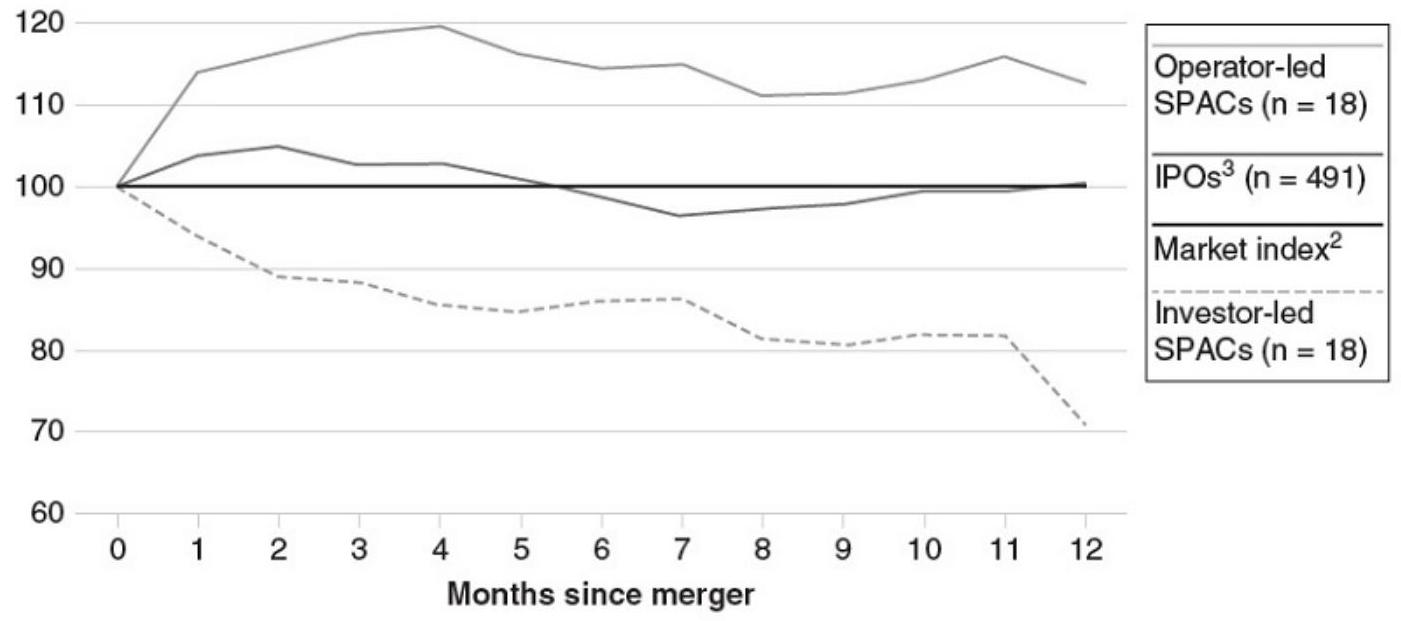
\includegraphics[max width=\textwidth]{2024_04_10_a5ce63565cca064665e9g-8}
\end{center}

Special-purpose acquisition companies with operators at the helm outperformed others.

${ }^{1}$ SPACs = special-purpose acquisition companies. Data covers 36 SPACs of $\geq \$ 200$ million that successfully merged during 2015-2019 and have 12 months of trading history.

${ }^{2}$ Refers to S\&P 500 sector indexes (e.g., for healthcare or consumer-discretionary sector) matched to IPO's sector. SPACs were compared with S\&P 600 midcap-sector indexes to reflect smaller company size.

${ }^{3}$ IPOs were compared with S\&P 500 sector indexes and do not include investment funds (eg, SPACs exchange-traded funds, real-estate investment trusts).

Source: S\&P Captial IQ; Mckinsey analysis

Source: Kurt Chauviere and Tao Tan, Earning the premium: A recipe for long-term SPAC success. McKinsey and Co, September 2020.

How can SPACs be structured to provide greater value to the long-term shareholders of private companies? When evaluating a SPAC, investors and private companies need to consider the dilution features of the structure. As previously shown, due diligence regarding the experience of the sponsor should be conducted, as operator-led SPACs may outperform SPACs led by financiers. The track record of the sponsor should be evaluated to see how many prior companies the sponsor has purchased or taken public, including the after-market performance of those companies. The structure of the sponsor promote is also important, as sponsors taking less than $20 \%$ promote or the sponsor and PIPE investors agreeing to lockup periods of one year or longer may contribute to lower dilution and higher aftermarket returns. The redemption structure also impacts the dilution, because allowing cash to be withdrawn from the SPAC before the business combination is completed increases dilution by requiring new financing, often at terms more favorable than those for existing shareholders. Finally, the warrant ratio matters, because units including one warrant cause much more dilution than units including between 0.25 and 0.5 warrants per share. SPACs issued in 2020 were more likely to include 0.5 warrants or fewer, while warrant structures were more lucrative in the past.

The degree of dilution is reduced as the value of the business combination increases relative to the size of the IPO of the SPAC. If the enterprise value of the merged public company is three to four times the value of the funds raised in the SPAC's IPO, the warrants and founder's shares are a smaller portion of the company's value. Additional funds are raised through debt or other securities offerings to support the value of the newly public operating company.

Perhaps the most investor-friendly SPAC issued is the Pershing Square Tontine Holdings. ${ }^{10}$ Squire, Kenneth, Bill Ackman and Tontine Holdings Rewrite the Rules for SPACs (July 2020), \href{http://CNBC.com}{CNBC.com}. These units include warrants on one-ninth of a share that can be kept by redeeming shareholders and an additional warrant on twoninths of a share that can only be kept by shareholders maintaining the stock position until after the business combination has been completed. This structure also has very low promote, where Pershing Square can only exercise the $6.21 \%$ stake held through purchased warrants after shareholders have earned a $20 \%$ return. Tontines are annuities that pay a regular income to all surviving investors, while the shares of investors who have died are given to the surviving investors. The Pershing Square SPAC has tontine-like features, where the warrants forfeited by redeeming shareholders are reallocated to shareholders who continue to hold the SPAC beyond the time of the completion of the de-SPAC transaction.

\section*{Comparing SPACs, IPOs, and Direct Listings}
While SPACs, IPOs, and direct listings all reach the goal of a company becoming publicly traded, they each accomplish this goal with different costs, speeds, benefits, and drawbacks.

Gahng et al. compare the costs of going public via SPACs, IPOs, and direct listings. The costs noted in the exhibit Costs to Go Public Using SPACs, IPOs, and Direct Listings include underwriting fees, as well as warrants and promote and the first-day price increase for IPOs. Note that this does not include legal and regulatory fees.

Costs to Go Public Using SPACs, IPOs, and Direct Listings

\begin{center}
\begin{tabular}{|l|c|c|l|}
\hline
 & SPAC & IPO & Direct Listing \\
\hline
Median Cost/Market Cap & $14.1 \%$ & $4.8 \%$ & $0.3 \%$ \\
\hline
Median Cost/Proceeds & $50.4 \%$ & $28.4 \%$ & N/A \\
\hline
\end{tabular}
\end{center}

Source: Gahng, Ritter, and Zhang, SPACs, 2021 Working Paper, University of Florida.

Direct listings are likely to be the cheapest and the fastest way to go public. Direct listings are likely to be most effective for brand-name firms, where their large public customer base gives them the name recognition to create a new class of shareholders. Direct listings typically do not include the research and fundraising support of an underwriter or the managerial expertise of a SPAC sponsor.

We see that SPACs may be a significantly more expensive way to go public than either an IPO or a direct listing, largely due to the dilution created through the warrants and the sponsors promote. What benefits do companies get from merging with a SPAC that may justify these higher costs? First, we note that the IPO process takes many months and does not have any certainty regarding the IPO price or even whether the deal will happen until the day of the IPO or the day before. In contrast, SPACs may take a company public more quickly with greater certainty on the valuation and probability of going public. While the IPO process waits for a large number of investors to make a financial commitment, the SPAC sponsor and private company can sign a definitive contract that guarantees the price and time of closing. Of course, the contract between the SPAC sponsor and the private company must be approved by a vote of the shareholders of the SPAC.

Private companies may also wish to go public using the SPAC structure when they can benefit from a relationship with a sponsor who can provide management assistance from a sponsor with a successful track record in their specific industry.

Finally, private companies may find that going public via a SPAC may be their only option, because some companies would not be qualified to float an IPO. While the IPO prospectus requires a statement of historical financials and risk factors of the firm, the IPO of the SPAC has limited disclosures, because it is only the shell company of the SPAC that is being taken public. By definition, the SPAC has no historical financials and no risk factors because the target company has not yet been identified. When the SPAC names the portfolio company, the business combination is now governed by regulations on mergers, not IPOs. At the time of the proposed business combination, SPAC sponsors can provide up to three years of forward-looking financial projections, many of which have been highly speculative. For example, a number of electric vehicle and battery companies with little to no historical revenue went public through combinations with SPACs in 2020. Some of those companies projected revenues of over $\$ 1$ billion in just three years. The public market seems to have accepted these financial projections and valued the stocks as if those revenue targets had already been attained. Some say, then, that companies going public via SPACs today would be among those eligible to float traditional IPOs three years from now.

\begin{itemize}
  \item 
\end{itemize}


\end{document}